%%%%%%%%%%%%%%%%%%%%%%%%%%%%%%%%%
\subsection{Raster Graphics}

Raster images are the simple matrix representation of an image. A raster image is conceptually a matrix of pixels, or a bitmap. Each pixel may contain multiple data points representing channels (colors). Historically, bitmaps have been the dominant representation for images due to their conceptual simplicity and the array-based display (and framebuffer) of modern screen technology. Much effort has been spent in enhancing the compression (e.g., lossy JPEG compression vs. lossless PNG compression) and analysis of raster images. Many image analysis methods depend on the grid-like representation of raster images, such as in the case of efficient parallel computation. Standardized raster images tend to have better support than vector graphics on older devices.

%%%%%%%%%%%%%%%%%%%%%%%%%%%%%%%%%
\subsection{Vector Graphics}

Vector graphics are not represented as pixels, but rather as a collection of parameterized geometric shapes. One of the immediate benefits is an efficient representation for purely geometric images, and the efficient and perfect scaling of continuous geometric objects. In order to display a vector image onto a pixel-based screen, the vector image first has to be rasterized, or rendered. Vector graphics are especially useful for web graphics and other highly geometric designs, such as maps, CAD, and typography. However, vector-based designs tend to be more inefficient for arbitrary image data (with high entropy), due to the relative complexity of shapes to pixels.

%%%%%%%%%%%%%%%%%%%%%%%%%%%%%%%%%
\subsection{Scalable Vector Graphics File Format}

Scalable Vector Graphics, or SVG, is a standard for vector graphics that uses the XML text format. All elements are represented using combinations of seven geometric shapes: Path, Rectangle, Circle, Ellipse, Line, Polyline, and Polygon. Since it is a textual format, it can be easily examined and manipulated by computers or by humans. The SVG standard is stable and supported by many applications, including PDF viewers and web browsers.

%%%%%%%%%%%%%%%%%%%%%%%%%%%%%%%%%
\subsection{Content Loss}

Content loss was introduced in \customcite{dumoulin2017learned}. The purpose of content loss is to quantify the difference in content between two images. Content loss was introduced as a loss function to train generative adversarial networks for style transfer.

The authors define the content loss between two images as the Euclidean distance between the high-level outputs of a trained classifier. This stems from a theory about deep convolutional neural networks: the early layers in a classifier are used to extract low-level features, such as edges, while the later layers of the classifier use the low-level features to create high-level features, such as an arm or a leg.

We tested the content loss metric on three images related to style transfer. The images were from \url{https://www.tensorflow.org/tutorials/generative/style_transfer}. 

\begin{figure}[H]
    \centering
    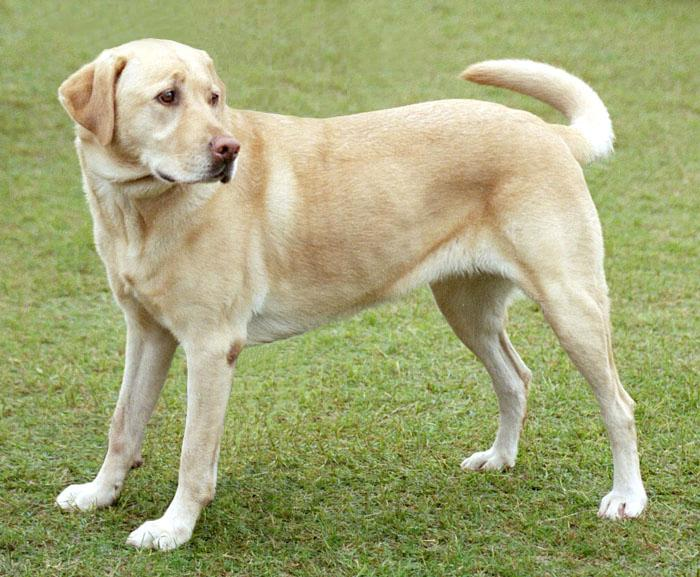
\includegraphics[width=\linewidth]{Figures/content_loss_images/lab1.jpg}
    \caption{\href{https://commons.wikimedia.org/wiki/File:YellowLabradorLooking_new.jpg}{Yellow Labrador Looking}, from Wikimedia Commons}
    \label{fig:lab_original}
\end{figure}

\begin{figure}[H]
    \centering
    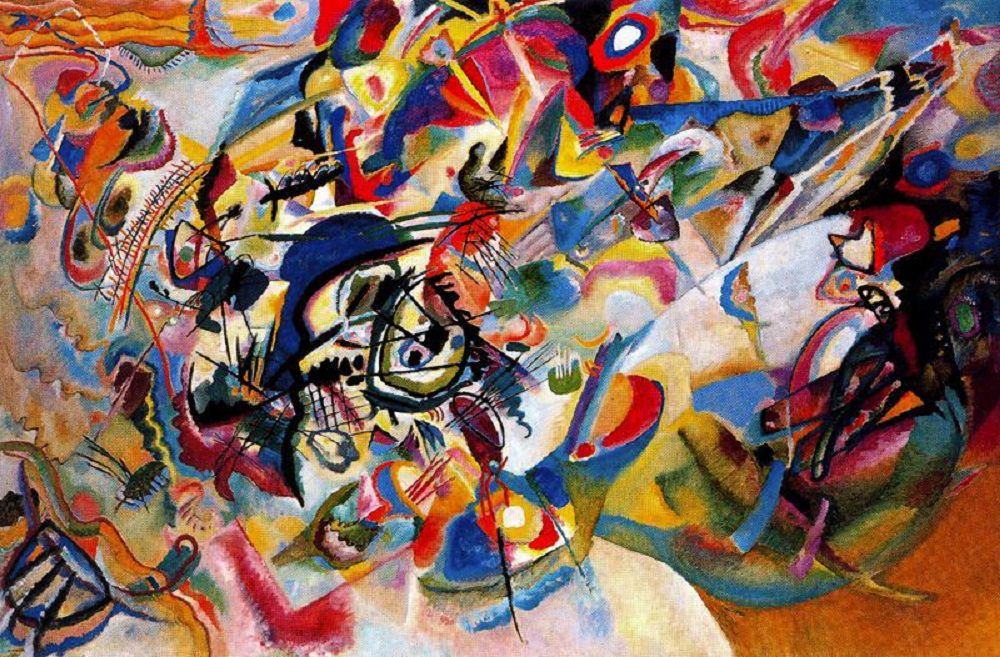
\includegraphics[width=\linewidth]{Figures/content_loss_images/lab2.jpg}
    \caption{Composition VII by Wassily Kandinsky}
    \label{fig:lab_style}
\end{figure}

\begin{figure}[H]
    \centering
    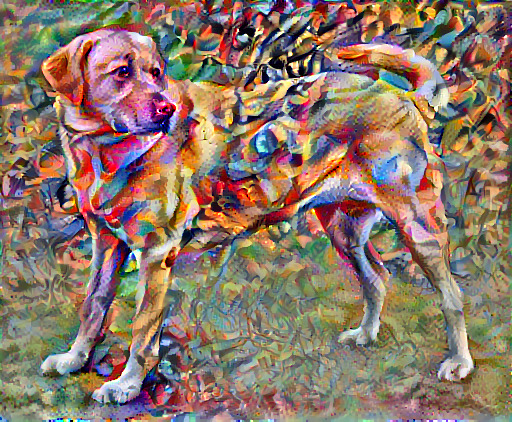
\includegraphics[width=\linewidth]{Figures/content_loss_images/lab3.jpg}
    \caption{Generated image produced with style transfer}
    \label{fig:lab_style_transfer}
\end{figure}

\cref{fig:lab_style_transfer} is generated using the content from \cref{fig:lab_original} and the style from \cref{fig:lab_style}. The content loss between \cref{fig:lab_original} and \cref{fig:lab_style_transfer} should be the lowest, compared to the content loss between \cref{fig:lab_original} and \cref{fig:lab_style}, because the two images have the same content but with different style. 
